\documentclass[twoside,11pt,a4paper]{book}


\linespread{1.1}
\usepackage{scribepkg}

%% Local Macros and packages: add any of your own definitions here.
\usepackage{amsmath,tikz}
\usetikzlibrary{bayesnet}
\newcommand{\data}[1]{\mathbf{#1}}
\renewcommand\thesection{\arabic{section}}

\begin{document}

\lecture{11 : Discrete Latent Variable Models}{Sanmi Koyejo}{Raj Kataria, Amit Das, Sep. 27, 2016} % Lecture name, Lecturer, Scribes

% ===========================
\section{Mixture Models}
Mixture models are used for representing data when they appear in clusters. Here, each cluster represents a \textit{mixture} or a \textit{component}. There is one model per component (or cluster) which we will refer to as a \textit{component model}. The collection of all component models leads to the formation of richer model called the \textit{mixture model}.

% ---------------------------
\subsection{Representation}
We assume that a mixture model can be represented as a directed graphical model as shown in Figure \ref{fig:DAG-MM}.
\begin{figure}[ht]
\centering
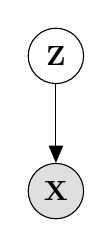
\begin{tikzpicture}
  % Define nodes
  \node[latent] (Z) {$\mathbf{Z}$};
  \node[obs, below=of Z] (X) {$\mathbf{X}$};

  % Connect the nodes
  \edge {Z} {X} ;  
\end{tikzpicture}
\caption{Directed Graphical Model representing a Mixture Model}
\label{fig:DAG-MM}
\end{figure}


Here, $X$ is the observed random variable representing the data and $Z$ is the hidden (or latent) random variable representing the component. Together, they represent a generative model where the observed data point $X$ is generated from the component (cluster index) $Z$. In general, $X$ and $Z$  can be continuous or  discrete. However, in this lecture, since we are dealing with \textit{discrete} latent variable models, we will assume $Z$ is discrete. The assumption that $Z$ is hidden is also valid since just by observing at $X$, it is hard to infer which component (or cluster) model generated $X$.

Assume $\data{X} \in \mathbb{R}^{d}$ is an observed $d$-dimensional random vector and $Z \in \{1, 2, \cdots, K\}$ where $K$ represents the number of components (or clusters). Therefore, the mixture model can be mathematically represented as,
\begin{align}
p(\data{X}) = \sum_{Z = 1}^{K} p(\data{X}, Z) &= \sum_{Z = 1}^{K} p(Z) p(\data{X}|Z), \label{eq:MixModel}
\end{align}
where,
\begin{align}
\sum_{Z = 1}^{K} p(Z) &= 1. \label{eq:Zsumto1}
\end{align}
The equation in \eqref{eq:MixModel} is the mixture model equation. It is simply alluding to the fact that we do not know for sure which individual component out of $K$ components generated the data point $\data{X}$ (since $Z$ is hidden). Then the data point can be assumed to be generated by a rich mixture model which is a collection of individual component models $p(\data{X}|Z)$ where each component model contributes to the generation of data point. The contribution weights from the individual component models are determined by $p(Z)$. Thus, if a particular component has a higher weight than all the other $K - 1$ components, then it is more likely that the data point was generated by that component.


% ---------------------------
\subsection{Inference and Learning}
Two interesting problems associated with mixture models are the following:
\begin{itemize}
\item \textbf{Inference:} Given $\data{X}$, what is $p(Z|\data{X})$? The term $p(Z|\data{X})$ is the aposteriori probability that the observed data point $\data{X}$ was generated by component $Z$. This is simply,
\begin{align}
p(Z|\data{X}) &= \frac{p(\data{X}|Z)p(Z)}{p(\data{X})}, \label{eq:ZgivenX}
\end{align}
where $p(\data{X}|Z), p(Z), p(\data{X})$ are given in \eqref{eq:MixModel} and \eqref{eq:Zsumto1}.
\item \textbf{Learning:} The equation in \eqref{eq:ZgivenX} cannot be solved unless we know \eqref{eq:MixModel} and \eqref{eq:Zsumto1}. Thus, the learning problem involves finding $p(Z)$ and $p(\data{X}|Z)$. A few approaches for addressing this problem are the following:
\begin{itemize}
\item Theory and statistics.
\item Learning model parameters assuming that the model is part of a family of distributions.
\item Learning without making any distribution assumptions. This falls into the category of learning non-parametric distributions.
\end{itemize}
In this lecture, we are interested in the second approach, i.e., learning the model parameters of a family of distributions.
\end{itemize}


% ---------------------------
\subsection{Learning Mixture Models Using Parametric Distributions}
In this section, we formulate the general framework of the learning problem involving parametric distributions.

Instead of representing a data point as $X$ as we have been doing so far, we'll represent the $i^{th}$ data point as $\data{X}_{i}$. Thus, for $N$ i.i.d. observed data points $\data{X}_{1}, \data{X}_{2}, \cdots, \data{X}_{N}$, we have their corresponding latent variables $Z_{1}, Z_{2}, \cdots, Z_{N}$. The directed graphical model for this case is shown in Figure \ref{fig:DAG-MM-IID}
\begin{figure}[ht]
\centering
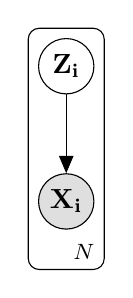
\begin{tikzpicture}
  % Define nodes
  \node[latent] (Z) {$\mathbf{Z_{i}}$};
  \node[obs, below=of Z] (X) {$\mathbf{X_{i}}$};

  % Connect the nodes
  \edge {Z} {X} ;
  
  % Plates
  \plate {ZX} {(Z)(X)} {$N$} ;
\end{tikzpicture}
\caption{Directed Graphical Model representing a Mixture Model for $N$ i.i.d. data points $\data{X}_{i}$, where $i = 1, \cdots, N$. The corresponding hidden variables are given by $Z_{i}$. The independence of $N$ observations is indicated by the plate.}
\label{fig:DAG-MM-IID}
\end{figure}

The joint denisty of the observed and latent variables is given by,
\begin{align}
p(\data{X}_{1}, \data{X}_{2}, \cdots, \data{X}_{N},Z_{1}, Z_{2}, \cdots, Z_{N}) & \stackrel{\text{i.i.d.}}{=} \prod_{i=1}^{N} p(\data{X}_{i}, Z_{i}). \label{eq:jointdensityiid}
\end{align}

The mixture model equation for \eqref{eq:jointdensityiid} is obtained by marginalizing \eqref{eq:jointdensityiid} over $Z_{1}, Z_{2}, \cdots, Z_{N}$. Thus,
\begin{align}
p(\data{X}_{1}, \cdots, \data{X}_{N}) &= \sum_{Z_{1}, ... , Z_{N}} p(\data{X}_{1}, \cdots, \data{X}_{N},Z_{1}, \cdots, Z_{N}) \nonumber \\
 & \stackrel{\eqref{eq:jointdensityiid}}{=} \sum_{Z_{1}, ... , Z_{N}} \prod_{i=1}^{N} p(\data{X}_{i}, Z_{i}) \nonumber \\
 & = \prod_{i=1}^{N} \sum_{Z_{i}} p(\data{X}_{i}, Z_{i}) \nonumber \\
&  \stackrel{\eqref{eq:MixModel}}{=} \prod_{i=1}^{N} \sum_{Z_{i}} p(Z_{i}) p(\data{X}_{i}|Z_{i}) \label{eq:MixModeliid0}
\end{align}
Since we are dealing with parametric distributions, we will parameterize $p(\data{X}_{1}, \cdots, \data{X}_{N})$ in \eqref{eq:MixModeliid0} with a set of parameters $\{\bm{\theta}_{1}, \bm{\theta}_{2}, \cdots, \bm{\theta}_{K}\}$, where each $\bm{\theta}_{k}$ represents a smaller set of parameters corresponding to component $k$ where $k \in \{1, \cdots, K\}$. Moreover, we define $p(Z_{i} = k) \stackrel{\Delta}{=} \pi_{k}$ as the prior for component $k$. Thus, $\pi = \{\pi_{1}, \cdots, \pi_{K}\}$ represents the prior distribution over the $K$ components. As a result, the entire parameter set consists of $\bm{\theta} = \{\pi_{k}, \bm{\theta}_{k}\}$, where $k = 1, \cdots, K$. Thus, incorporating the model parameters $\bm{\theta}$ in \eqref{eq:MixModeliid0},  \eqref{eq:MixModeliid0} can be written as,
\begin{align}
p(\data{X}_{1}, \cdots, \data{X}_{N}; \bm{\theta}) &= \prod_{i=1}^{N} \sum_{Z_{i}} p(Z_{i} = k) p(\data{X}_{i}|Z_{i} = k; \bm{\theta}_{k}) \nonumber \\ 
&= \prod_{i=1}^{N} \sum_{Z_{i}} \pi_{k} p(\data{X}_{i}|Z_{i} = k; \bm{\theta}_{k}) \label{eq:MixModeliid}
\end{align}
For the special case of $i=1$, \eqref{eq:MixModeliid} becomes \eqref{eq:MixModel} when parameterized by $\bm{\theta}$. 

The objective of the learning problem is to estimate the parameters $\bm{\theta}$ such that the likelihood of the mixture model in \eqref{eq:MixModeliid} is maximized. Thus,
\begin{align}
\bm{\theta}^{\star} &= \argmax_{\bm{\theta}} \ p(\data{X}_{1}, \cdots, \data{X}_{N}; \bm{\theta}) \nonumber \\
                    &= \argmax_{\bm{\theta}} \ \text{log} \ p(\data{X}_{1}, \cdots, \data{X}_{N}; \bm{\theta}) \label{eq:MixModelLearningProblem}
\end{align}


% ---------------------------
\subsection{Gaussian Mixture Model}
Consider the component model $p(\data{X}_{i}|Z_{i} =k; \bm{\theta}_{k})$ in \eqref{eq:MixModeliid}. For the special case that each component in $p(\data{X}_{i}|Z_{i} = k; \bm{\theta}_{k})$ can be modeled by a Gaussian distribution, the mixture model in \eqref{eq:MixModeliid} becomes a Gaussian Mixture Model (GMM). Thus, for a given component $Z_{i} = k$, the component model can be represented as,
\begin{align}
p(\data{X}_{i}|Z_{i} = k; \bm{\theta}_{k}) = \mathcal{N}(\data{X}_{i}|Z_{i} = k; \bm{\theta}_{k} = (\bm{\mu}_{k}, \bm{\Sigma}_{k}) ), \label{eq:GaussianComponent}
\end{align}
where $\bm{\mu}_{k} \in \mathbb{R}^{d}$ is the mean and $\bm{\Sigma}_{k}$ is the $d \times d$ covariance matrix parameterizing the Gaussian component model in \eqref{eq:GaussianComponent}.
Note that, in the right hand side of \eqref{eq:GaussianComponent}, the parameter set is represented as $\bm{\theta}_{k}$ instead of $\bm{\theta}$. This is because for a given component $Z_{i} = k$, the component model is entirely determined by the parameters in $\bm{\theta}_{k}$. The parameters of the other components $\bm{\theta}_{j}$, $j \ne k$, do not determine the value of the probability in \eqref{eq:GaussianComponent}. However, there is nothing wrong in using the notation $\mathcal{N}(\data{X}_{i}|Z_{i} = k; \bm{\theta})$ instead of $\mathcal{N}(\data{X}_{i}|Z_{i} = k; \bm{\theta}_{k})$. The former notation may be used in some textbooks. When the former notation is used, it must be implicitly understood that only $\bm{\theta}_{k} \subseteq \bm{\theta}$ is used to evaluate \eqref{eq:GaussianComponent}. Other parameters in $\bm{\theta}$ are not used to evaluate \eqref{eq:GaussianComponent}.

The other term $p(Z_{i} = k) = \pi_{k}$ in \eqref{eq:MixModeliid} is the prior probability of component $k$. Thus, the GMM for the data point $\data{X}_{i}$, can be written as,
\begin{align}
p(\data{X}_{i}; \bm{\theta}) &= \sum_{Z_{i}} \pi_{k} \mathcal{N}(\data{X}_{i}|Z_{i} = k; \bm{\theta}_{k} = (\bm{\mu}_{k}. \bm{\Sigma}_{k}) ) \nonumber \\ 
&= \sum_{Z_{i}} \pi_{k} \mathcal{N}(\data{X}_{i}; \bm{\theta}_{k} = (\bm{\mu}_{k}. \bm{\Sigma}_{k}) )
\label{eq:GMM1}
\end{align}
where,
\begin{align}
\mathcal{N}(\data{X}_{i}; \bm{\theta}_{k} = (\bm{\mu}_{k}. \bm{\Sigma}_{k}) ) &= \frac{1}{(2\pi)^{d/2} |\Sigma_{k}|^{\frac{1}{2}}} \exp{\Bigg(\frac{-1}{2}(\bm{x}_{i} - \bm{\mu}_{k})^{T}\bm{\Sigma}_{k}^{-1}(\bm{x}_{i} - \bm{\mu}_{k})\Bigg)}.
\end{align}


The learning problem in GMM is to determine the parameters $\bm{\theta} = \{\pi_{k}, \bm{\mu}_{k}, \bm{\Sigma}_{k}\}$, where $k = 1, \cdots, K$. This can be obtained by substituting the individual Gaussian component model from \eqref{eq:GMM1} in \eqref{eq:MixModeliid} and the resulting equation in \eqref{eq:MixModelLearningProblem}. Thus, the GMM learning problem becomes,
\begin{align}
\bm{\theta}^{\star} &= \argmax_{\bm{\theta}} \ \text{log} \ p(\data{X}_{1}, \cdots, \data{X}_{N}; \bm{\theta}) \nonumber \\
&= \argmax_{\bm{\theta}} \sum_{i=1}^{N} \ \text{log} \Bigg( \sum_{k = 1}^{K} \pi_{k} \mathcal{N}(\data{X}_{i}; \bm{\theta}_{k}) \Bigg) \label{eq:GMMLearningProblem}
\end{align}


The total number parameters to be estimated in \eqref{eq:GMMLearningProblem} is $K + Kd + K\frac{d (d+1)}{2}$. Due to the symmetric nature of covariance matrices, the maximum number of parameters per covariance matrix is $\frac{d (d+1)}{2}$. Finding the optimal $\bm{\theta}^{\star}$ in \eqref{eq:GMMLearningProblem} is a $d$-dimensional non-concave optimization problem. It is hard to find a globally optimum solution $\bm{\theta}^{\star}$ directly. In the next class, we will see how a sub-optimal solution can be obtained using the Expectation-Maximization (EM) algorithm \cite{Dempster-EM}. It is sub-optimal because it is guaranteed to find a locally optimal value of $\bm{\theta}$ but not guaranteed to find the global optimum $\bm{\theta}^{\star}$.

Here, we'll introduce the term $\tau_{k}^{i}$ which will be used during EM. For an observed data point $\data{X}_{i}$, $\tau_{k}^{i}$ is the aposteriori probability that the data point $\data{X}_{i}$ was generated by component $k$. Thus,
\begin{align}
\tau_{k}^{i} & \stackrel{\Delta}{=} p(Z_{i} = k|\data{X}_{i}; \bm{\theta}) \nonumber \\
         &=  \frac{p(\data{X}_{i}|Z_{i} = k; \bm{\theta}_{k}) p(Z_{i} = k)}{p(\data{X}_{i}; \bm{\theta})} \nonumber \\
         &= \frac{\pi_{k} \mathcal{N}(\data{X}_{i}; \bm{\theta}_{k} = (\bm{\mu}_{k}. \bm{\Sigma}_{k}) )}{\sum_{j=1}^{K} \pi_{j} \mathcal{N}(\data{X}_{i}; \bm{\theta}_{j} = (\bm{\mu}_{j}. \bm{\Sigma}_{j}) )}
\end{align}


% ---------------------------
\subsection{Determining the number of components ($K$) in a Mixture Model}
There are a number of ways to determine the number of components $K$.
\begin{itemize}
\item With increasing values of $K$, the log likelihood score,  $\text{log} \ p(\data{X}_{1}, \cdots, \data{X}_{N}; \bm{\theta})$ in \eqref{eq:MixModelLearningProblem} increases. However, after a certain value of $K$, the increase in score is marginal. Thus, if the \textit{increase} in score becomes less than some heuristically determined threshold, then we stop increasing $K$.
\item The model complexity is a function of $K$ and can be determined by AIC (Akaike Information Criterion) or BIC (Bayesian Information Criterion). Both AIC and BIC increase when $K$ increases. Thus, by using a modified cost function where the original cost function is penalized by AIC or BIC, the model complexity can be controlled. This is given as,
\begin{align}
\bm{\theta}^{\star} &= \argmax_{\bm{\theta}} \Big\{ \ - \text{log} \ p(\data{X}_{1}, \cdots, \data{X}_{N}; \bm{\theta}) + C(\bm{\theta}) \Big\}
\end{align}
\item Another way to control $K$ is by using the out-of-sample fit method. Here, for each $\bm{\theta}_{k}$,  we evaluate the likelihood of data points from a cross-validation set that is not present during training. If the likelihood of the cross-validation set increases more than a heuristically set threshold, we increase $K$. Else, we do not increase $K$ any further.
\end{itemize} 
% ===========================

\bibliographystyle{ims}
\bibliography{scribe}


\end{document}

